
This chapter presents the chosen case study, which serves as a stimulus for system design and demonstrates 
the practical application of the developed work. The chosen case study focuses on the \gls{crc} peripheral,
which is present in several microcontroller families, such as STM32 \cite{referenceManualRM0385} or Xilinx Zynq \cite{xilinx2014zynq} 
nevertheless, the VExpress\_gem5, which is a board introduced by Gem5, does not have it.

The \gls{crc} was created in 1961 by William Wesley Peterson \cite{peterson1961cyclic}. As the name suggests, 
it utilizes systematic cyclic codes to encode messages by incorporating a fixed-length check value. In the end, his work
contributed significantly to simplifying and enhancing the detection of accidental errors/changes in communication 
networks. \gls{crc} uses a generator polynomial, which is known by the sender and receiver, and it is used to 
perform the calculation. There are different standards however, the most common ones are the CRC-8, CRC-12, CRC-16, 
CRC-32, and CRC-CCIT \cite{borrelli2001ieee}

Another application for the \gls{crc} is the storage integrity. Due to defective components or electromagnetic fields,
bits can change their value without notice. In the presented case study, this scenario will be explored, where 
the \gls{crc} peripheral is used to maintain a specific memory state and verify if there have been any changes. 
Furthermore, to showcase the advantages of the previously developed work, the application will perform other 
tasks simultaneously. 

\section{CRC peripheral} %Software development

As mentioned earlier in this dissertation, co-simulation involves the integration of multiple simulation tools from different
domains. Because of that, it is required to develop a system that can execute and communicate among them. The following picture
demonstrates how the different tools will communicate with each other.

\begin{figure}[H]
	\centering
 	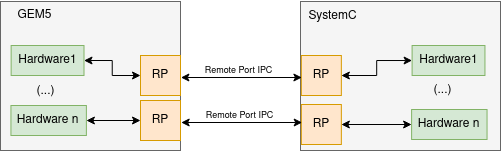
\includegraphics[width=0.8\linewidth]{Images/CoSimDesignSimplified.png} 
 	\caption{Co-simulation design}
	 \label{fig_CoSimDesignSimplified}
\end{figure}

The communication will be done using a remote port \gls{ipc}. This should be created and connected before the beginning of the
simulation, in a way that transactions occur. Each hardware device will have a unique connection to avoid concurrency problems.
It is important to remember that this hardware is not presented on the board, reason why is needed another simulator. The subsequent sections 
will delve into the detailed explanations of the \gls{crc} component. It's worth noting that the design process 
took significant reference from the STM32 microcontroller family's reference manual \cite{referenceManualRM0385}.


\subsection{SystemC}

The peripheral development was carried out using the SystemC tool. In this example, it will only simulate the \gls{crc} but, it has
the capability to simulate more than just one peripheral. For instance, picture a scenario where the workload also requires an \gls{adc}.
This device is also not included in the VExpress\_gem5 board, so it would also require its implementation. For this reason, flexibility
is a requirement, and with this idea in mind, the subsequent design was developed.

\begin{figure}[H]
	\centering
	\begin{subfigure}{0.45\textwidth}
		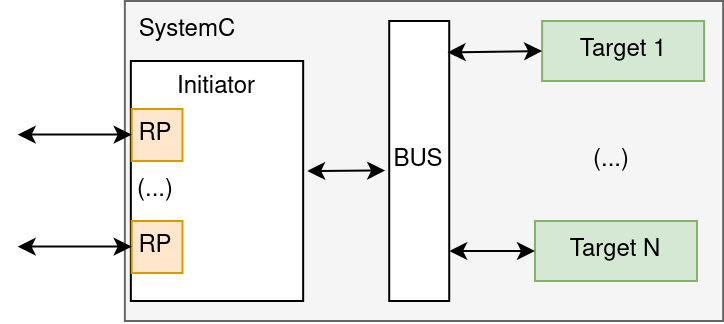
\includegraphics[width=\textwidth]{Images/SystemCdesign.png}
 		\caption{General SystemC design}
	 	\label{fig_SystemCdesign_geral}
	\end{subfigure}
	\hfill
	\begin{subfigure}{0.45\textwidth}
		\centering
		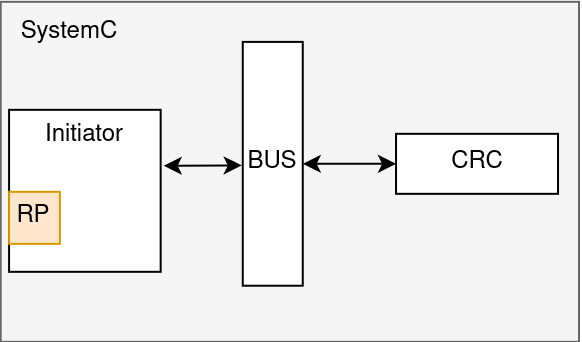
\includegraphics[width=\textwidth]{Images/SystemCdesign_CRC.png}
		\caption{SystemC design with CRC}
		\label{fig_SystemCdesign_CRC}
	\end{subfigure}
		
	\label{fig:SystemCsdesign}
\end{figure}


It is composed of three main components. The initiator, the bus, and the targets. Beginning with the first, it serves as the initial 
point of interaction for the tool, as it handles incoming frames received through the remote port. The remote port operates independently 
of the initiator, enabling asynchronous reception and transmission of bytes through the receiver and transmit buffers, respectively.
Additionally, it also performs an interpretation of the received trama and creates the \gls{tlm} transaction. It analyses various 
parameters such as the operation type, the desired target, and the memory region, among others, with the help of \gls{tlm} wrapper, 
which will presented in the \autoref{subsec::TLMwrapper}.

The bus is responsible for forwarding the \gls{tlm} transaction to the right target. Each target has a unique ID, that is attributed to it 
at the beginning of the simulation. Gem5's board is a 32-bit processor, meaning that each transaction is 32-bit in length. However, SystemC 
\gls{tlm} transactions can be 64-bit, leaving 32 bits unused. Before the transmission, the initiator uses these bytes to set the 
target\_ID, which will be utilized by the bus to identify the targets.

Lastly, the targets are the peripherals, that can be different from each other, as mentioned in the previous example. These receive the 
\gls{tlm} commands and act accordingly. Since in this dissertation, the focus will be the \gls{crc}, a single target will be implemented
thus, the \autoref{fig_SystemCdesign_geral} can be redefined to the \autoref{fig_SystemCdesign_CRC}. This will have the following
characteristics \cite{referenceManualRM0385}. 

\begin{itemize}
	\item Uses CRC-32 (Ethernet) polynomial: 0x4C11DB7
	\item Programmable CRC initial value
	\item Single input/output 32-bit data register
	\item CRC computation done in 4 clock cycles 
	\item General-purpose 8-bit register (can be used for temporary storage)
	\item Reversibility option on I/O data
\end{itemize}

\begin{figure}[]
	\centering
 	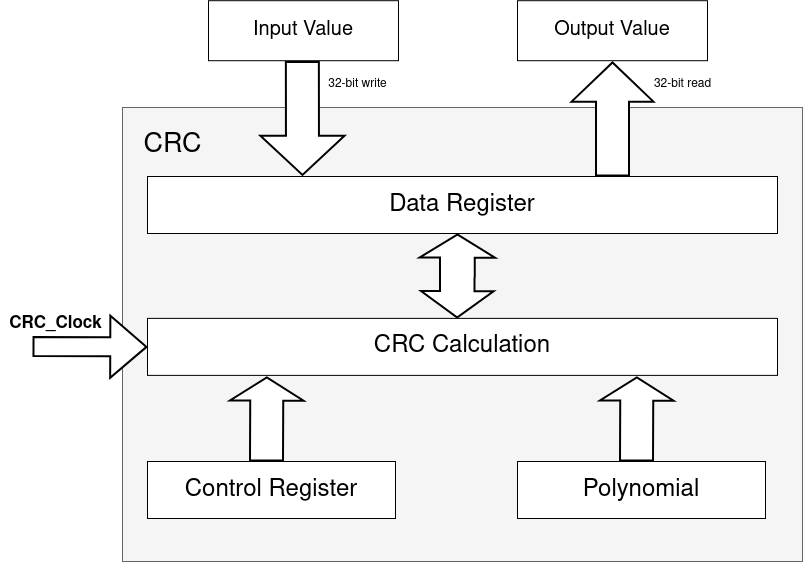
\includegraphics[width=0.6\linewidth]{Images/CrcBlockDiagram.png}
 	\caption{CRC block diagram}
	 \label{fig_CrcBlockDiagram}
\end{figure}

The peripheral will work as demonstrated in \autoref{fig_CrcBlockDiagram}. First of all, the user needs to write the input value 
in the data register (CRC\_DR). After four \gls{crc} clock cycles, the correspondent \gls{crc} value is fully calculated, and its
value is stored in the CRC\_DR. In this case, the \gls{crc} frequency with be equal to the \gls{cpu}. The data width must be 32-bit, 
hence whether the user needs a \gls{crc} for five bytes, for example, two different computations will be needed. 

Moreover, the input and output data can be reversed, to manage the various endianness schemes. For the input data, the reverse operation 
is controlled by the REV\_IN[1:0] bits, and for the output data, the REV\_OUT bit is used. These, along with the reset bit used to 
reset the \gls{crc}, are located in the control register (CRC\_CR). This bit must be set by software, and it is automatically cleared by
the hardware. An example of a reverse operation can be found on \autoref{tab:CRC_REV}.

\begin{table}[!htb]
    \caption{Reverse operation}
    \begin{minipage}{.5\linewidth}
      \centering
      \subcaption{Input}
		\resizebox{\textwidth}{!}{%
		\begin{tabular}{lllll}
		\cline{1-4}
		\multicolumn{1}{|l|}{\cellcolor[HTML]{C0C0C0}{\color[HTML]{000000} REV\_IN[1:0]}} & \multicolumn{1}{l|}{\cellcolor[HTML]{C0C0C0}{\color[HTML]{000000} Input}} & \multicolumn{1}{l|}{\cellcolor[HTML]{C0C0C0}{\color[HTML]{000000} Reverse Action}} & \multicolumn{1}{l|}{\cellcolor[HTML]{C0C0C0}{\color[HTML]{000000} Reverse Input}} &  \\ \cline{1-4}
		\multicolumn{1}{|l|}{0 0} & \multicolumn{1}{l|}{0x1A2B3C4D} & \multicolumn{1}{l|}{Not affected} & \multicolumn{1}{l|}{0x1A2B3C4D} &  \\ \cline{1-4}
		\multicolumn{1}{|l|}{0 1} & \multicolumn{1}{l|}{0x1A2B3C4D} & \multicolumn{1}{l|}{Bit-reversal done by byte} & \multicolumn{1}{l|}{0x58D43CB2} &  \\ \cline{1-4}
		\multicolumn{1}{|l|}{1 0} & \multicolumn{1}{l|}{0x1A2B3C4D} & \multicolumn{1}{l|}{Bit-reversal done by half-word} & \multicolumn{1}{l|}{0xD458B23C} &  \\ \cline{1-4}
		\multicolumn{1}{|l|}{1 1} & \multicolumn{1}{l|}{0x1A2B3C4D} & \multicolumn{1}{l|}{Bit-reversal done by word} & \multicolumn{1}{l|}{0xB23CD458} &  \\ \cline{1-4}
		&  &  &  & 
		\end{tabular}%
        }
        \label{tab:CRC_REV_IN}
    \end{minipage}%
    \begin{minipage}{.5\linewidth}
        \centering
        \subcaption{Output}
		\resizebox{\textwidth}{!}{%
		\begin{tabular}{lllll}
		\cline{1-4}
		\multicolumn{1}{|l|}{\cellcolor[HTML]{C0C0C0}{\color[HTML]{000000} REV\_OUT}} & \multicolumn{1}{l|}{\cellcolor[HTML]{C0C0C0}{\color[HTML]{000000} Output}} & \multicolumn{1}{l|}{\cellcolor[HTML]{C0C0C0}{\color[HTML]{000000} Reverse Action}} & \multicolumn{1}{l|}{\cellcolor[HTML]{C0C0C0}{\color[HTML]{000000} Reverse Output}} &  \\ \cline{1-4}
		\multicolumn{1}{|l|}{0} & \multicolumn{1}{l|}{0x11223344} & \multicolumn{1}{l|}{Not affected} & \multicolumn{1}{l|}{0x11223344} &  \\ \cline{1-4}
		\multicolumn{1}{|l|}{1} & \multicolumn{1}{l|}{0x11223344} & \multicolumn{1}{l|}{Bit-reversal done by word} & \multicolumn{1}{l|}{0x22CC4488} &  \\ \cline{1-4}
		 &  &  &  & 
		\end{tabular}%
        }   
        \label{tab:CRC_REV_OUT}
    \end{minipage}
	\label{tab:CRC_REV} 
\end{table}

By default, the polynomial coefficients are defined by 0x4C11DB7 nevertheless, it can be fully programmable through the CRC\_POL register.
It is important to mention that modifications in this register when a \gls{crc} computation is ongoing are not permitted, as it would 
compromise the output value. To conclude the available registers, are missing the CRC\_INIT and CRC\_IDR, which are used to initialize 
the \gls{crc} calculator in the reset, and to hold a temporary 8-bit value related to \gls{crc} calculation, respectively. 

Summing up, the \autoref{fig_CRC_read} and \autoref{fig_CRC_write} demonstrate how the peripheral will behave depending on the defined settings and desired 
operation. Before any execution, offset/size out-of-bounds, and permissions are verified to maintain the device's integrity. The 
functionality of these parameters will be explained further. 

\begin{figure}[H]
	\centering
 	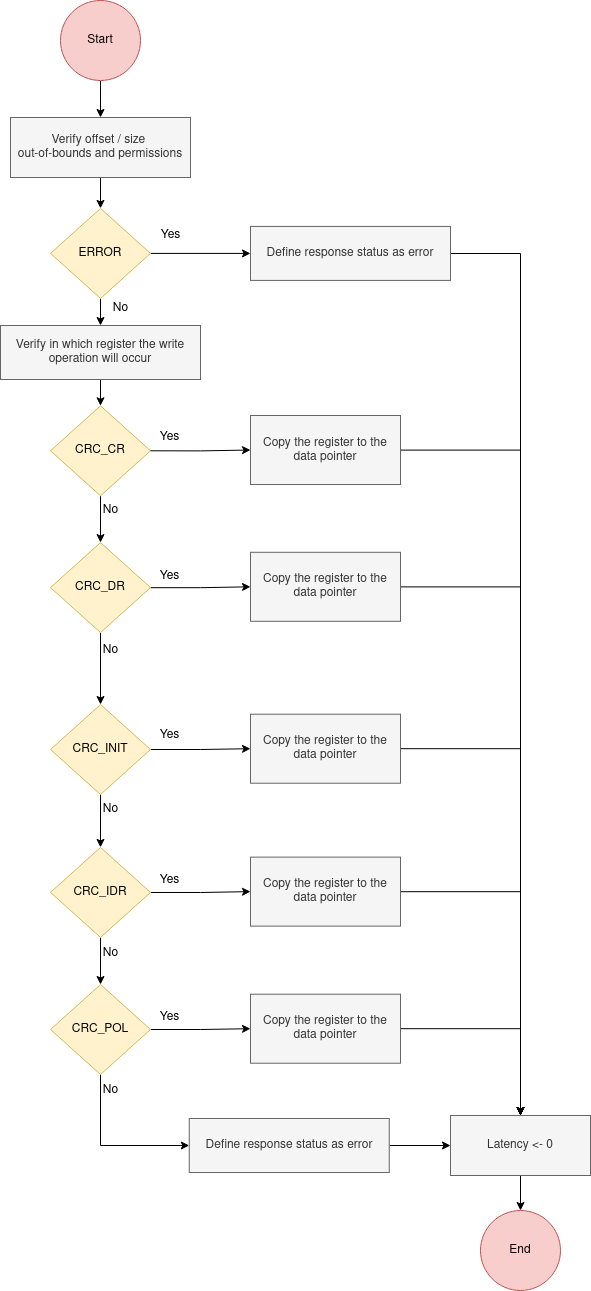
\includegraphics[width=0.8\linewidth]{Images/CRC_read.png} 
 	\caption{CRC read operation}
	 \label{fig_CRC_read}
\end{figure}

\begin{figure}[t!]
	\centering
 	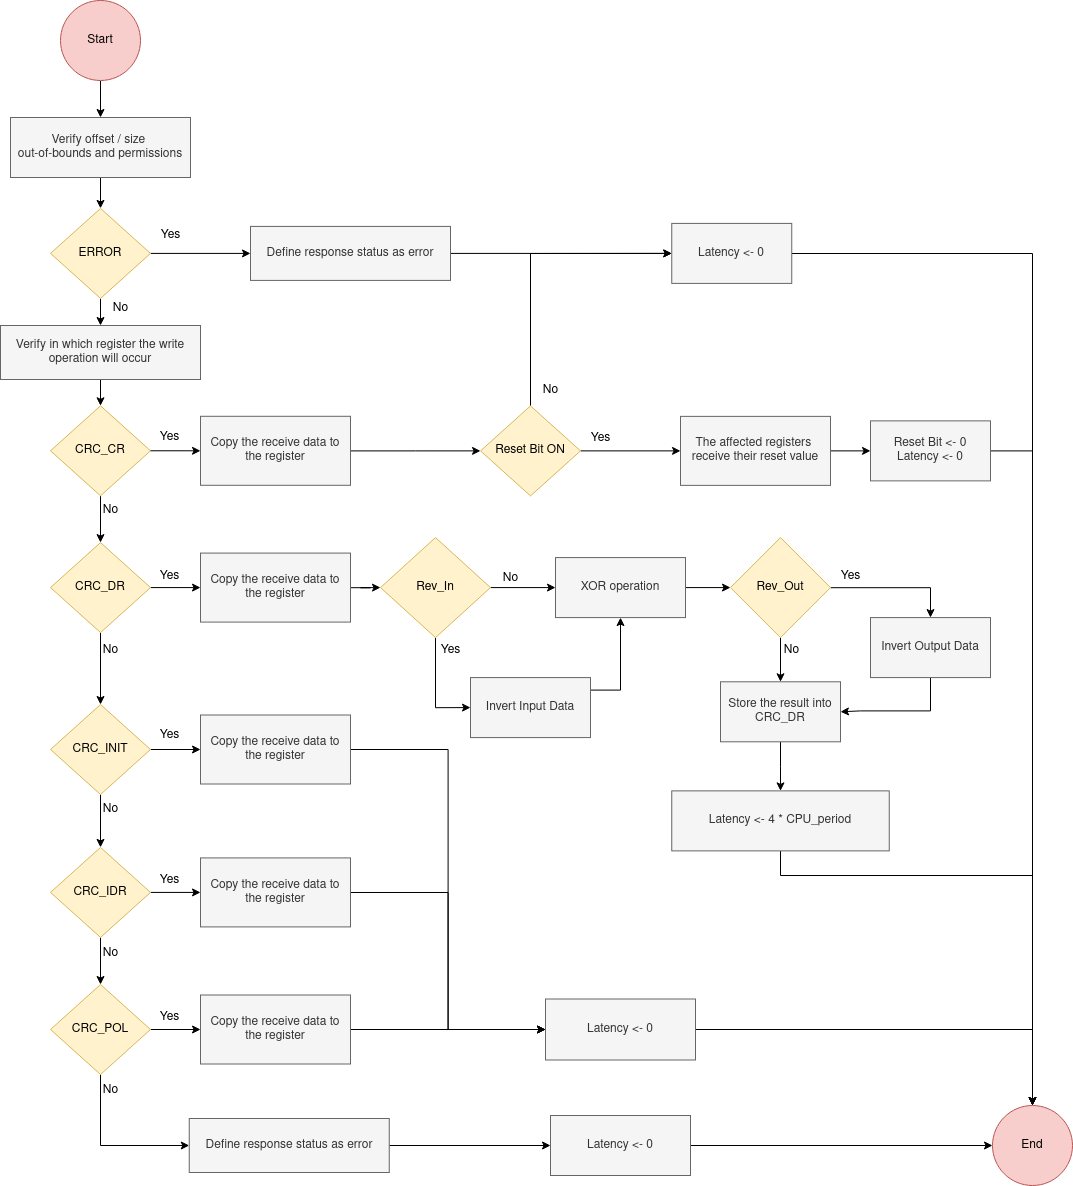
\includegraphics[width=0.7\linewidth]{Images/CRC_write.png}
 	\caption{CRC write operation}
	 \label{fig_CRC_write}
\end{figure}


\subsection{Gem5}

As aforementioned, Gem5 has available as a target platform the VExpress\_gem5 board. It is based on the ARM Versatile Express RS1, which 
consists of a motherboard and one or more daughterboards. The system provides a range of both on-chip and off-chip devices.
On-chip devices include the Generic Interrupt Controller (GIC), an LCD controller, and system timers.
Off-chip devices contain the Keyboard and Mouse Interface (KMI), Real-Time Clock (RTC), and \gls{uart}. 
The platform's memory map is divided into the next sections.

\def\mydots{\xleaders\hbox to0.25em{\hfill.\hfill}\hfill}

\begin{outline}[enumerate]
	\1 Boot memory 						\mydots 	0x00000000 to 0x03FFFFFF
	\1 Reserved							\mydots 	0x04000000 to 0x0FFFFFFF
	\1 Off-chip peripherals				\mydots 	0x10000000 to 0x1FFFFFFF
		\2 Gem5-specific peripherals	\mydots 	0x10000000 to 0x13FFFFFF
			\3 Energy controller 		\mydots 	0x10000000 to 0x1000FFFF
			\3 Pseudo-ops				\mydots		0x10010000 to 0x1001FFFF
			\3 MHU						\mydots		0x10020000 to 0x1002FFFF
		\2 Reserved 					\mydots 	0x14000000 to 0x17FFFFFF
		\2 VRAM							\mydots		0x18000000 to 0x19FFFFFF
		\2 Reserved 					\mydots		0x1A000000 to 0x1BFFFFFF
		\2 Peripheral block 1			\mydots		0x1C000000 to 0x1FFFFFFF
	\1 On-chip  peripherals				\mydots 	0x20000000 to 0x3FFFFFFF
	\1 PCI memory 						\mydots 	0x40000000 to 0x7FFFFFFF
	\1 DRAM								\mydots 	0x80000000 to 0xFFFFFFFF
\end{outline}

It is possible to notice that the Gem5-specific peripherals memory region is not fully occupied. Since the understudy device is 
not available on this board, its implementation will be done in this memory region. In accordance with the remaining devices, 
the memory from 0x10030000 to 0x1003FFFF will be reserved for SystemC \gls{crc}. Subsequently, it must be recognized as a Gem5 
peripheral to enable communication with it. To achieve this, it should be defined and added to the list of off-chip devices in the 
board's configuration. In addition, it is also required to create a \gls{pte} for the device, which can be done by following the
code on \ref{templatePTE}. However, it's important to note that even after this process, the \gls{crc} is only recognized as a device of the 
VExpress\_gem5 board and its implementation still need to be completed.

\hspace{1cm}

\begin{lstlisting}[style=customasm, caption={Template for a \gls{pte}}, label=templatePTE]
LDR   r1,= DEVICE_ADDR	 // CRC address -> 0x10030000
LSR   r1, r1, #20        // Find which 1MB block it is in
LSL   r2, r1, #2         // Gives offset into the page tables
LSL   r1, r1, #20        // Put back in address format
LDR   r3, =L1_DEVICE     // Descriptor template
ORR   r1, r1, r3         // Combine address and template
STR   r1, [r0, r2]       // Store table entry
\end{lstlisting}


\begin{figure}[t!]
	\centering
	\begin{subfigure}{0.4\textwidth}
		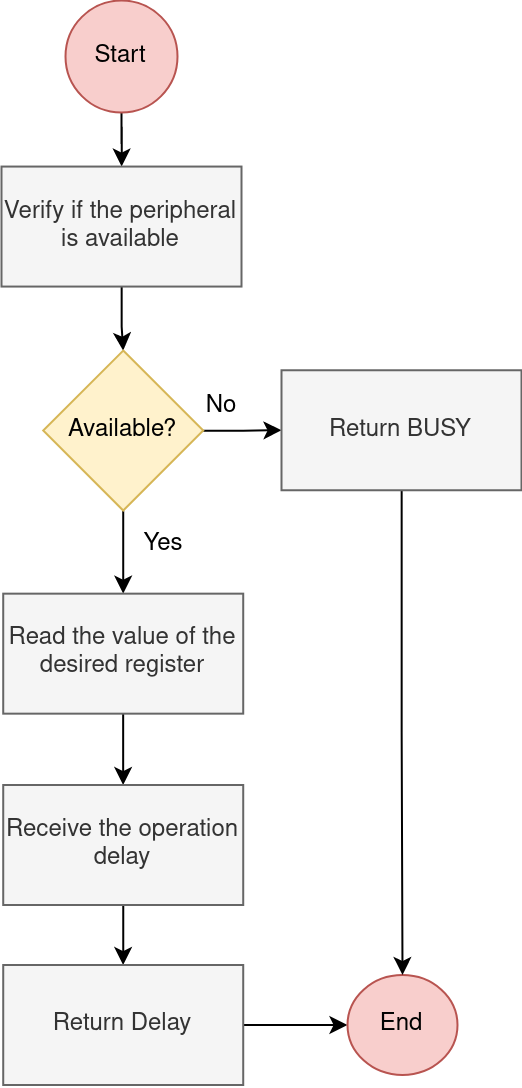
\includegraphics[width=0.7\textwidth]{Images/CrcReadFunction.png}
 		\caption[1\textwidth]{CRC read flowchart} 
	 	\label{fig_CrcReadFunction}
	\end{subfigure}
	\hspace{1cm}
	\begin{subfigure}{0.4\textwidth}
		\centering
		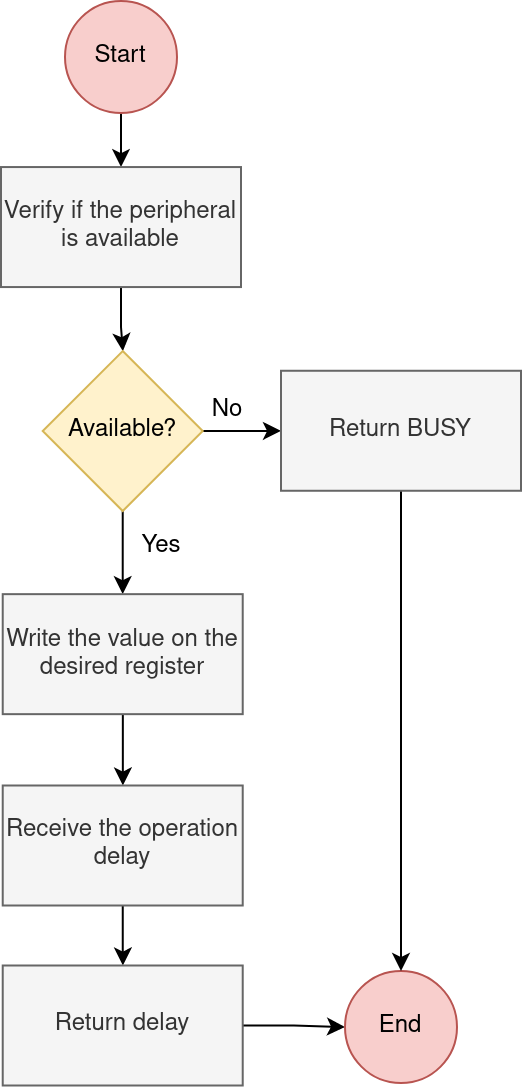
\includegraphics[width=0.7\textwidth]{Images/CrcWriteFunction.png}
		\caption[1\textwidth]{CRC write flowchart}
		\label{fig_CrcWriteFunction}
	\end{subfigure}
		
	\caption{Redefinition of \textit{BasicPioDevice} functions}
\end{figure}
 
To implement a device in Gem5, a few aspects are mandatory. First of all, the peripheral's Python interface. In this document, it is 
described the type, where implementation is, and, optionally, some parameters to be customized. In this context, these can be
the port number, for the remote connection, or the action time delay. In second place, is the implementation itself. Gem5 has implemented 
a device template, that is present in the class \textit{BasicPioDevice}. By inheriting this, the default configurations are placed 
nevertheless, read, and write functions still need to be defined, as these change from device to device. The figures \ref{fig_CrcReadFunction} and \ref{fig_CrcWriteFunction}
present its implementation. Further, other aspects must be present, like the \gls{crc} registers, the socket\_ID, and the remote 
port functions(listen, accept, and detach). The remote connection is done before the simulation starts, meaning that it does not
continue until a connection is made. As soon as it happens, an init function is called to state the initialization, with the 
device's information. It is required due to the possibility of various devices in SystemC. The last point is the \textit{Sconscript} file, 
which is required by the compiler to understand the available SimObjects. Here should be discriminated the SimObject, that is, 
the Python file, the SimObject's source file, and the debug flags, if presented.

\subsection{TLM wrapper}
\label{subsec::TLMwrapper}

Although Gem5 and SystemC are two frameworks that use C++, they cannot communicate directly with each other. Gem5 is unable to 
interpret the \gls{tlm} commands, just as SystemC doesn't understand read and write operations to the registers. For these reasons,
it is necessary a wrapper to enable communication between the two platforms. This will be available in both, and every transaction must
pass through it otherwise, the channel could be corrupted. 

\begin{figure}[H]
	\centering
 	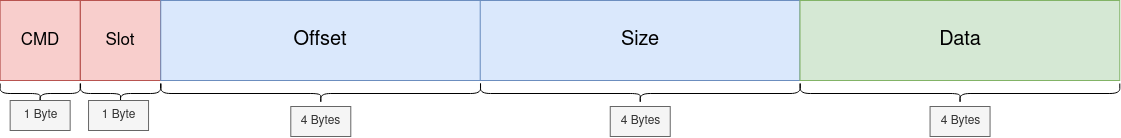
\includegraphics[width=0.8\linewidth]{Images/TLM_Wrapper_Payload.png} 
 	\caption{TLM wrapper payload definition}
	% \label{fig_TLM_Wrapper_Payload}
\end{figure}


The main part of the wrapper is the payload definition. It provides coherent communication between platforms, keeps the transactions
easy to understand, and improves efficiency. For this case, its definition can be found in the prior image. Each operation must 
have a command, a slot, reason why both have the color red. The remote port \gls{ipc} reads and writes eight bits at a time. 
Consequently, even if the command list does not use all the bits, a byte is allocated for their size. The list of commands can be found on
\autoref{tab_TLMwrapperCMD}. The slot is used as an ID. Regarding the \autoref{fig_CoSimDesignSimplified}, each peripheral has a remote 
connection associated hence, with this, is possible to decode the port where the transaction should be done. Offset and size are 
marked as blue since they are mandatory for both read and write operations. 
Data is with green color because only is necessary for the write action. Four bytes are demanded for these parameters, due to the 32-bit
processor present in the VExpress\_gem5 board.

\begin{table}[h!]
	\centering
	\begin{tabular}{lll}
	\cline{1-2}
	\multicolumn{1}{|l|}{\cellcolor[HTML]{C0C0C0}{\color[HTML]{000000} Bits}} & \multicolumn{1}{l|}{\cellcolor[HTML]{C0C0C0}{\color[HTML]{000000} Command}} &  \\ \cline{1-2}
	\multicolumn{1}{|l|}{00} & \multicolumn{1}{l|}{TLM\_INIT} &  \\ \cline{1-2}
	\multicolumn{1}{|l|}{01} & \multicolumn{1}{l|}{TLM\_CLOSE} &  \\ \cline{1-2}
	\multicolumn{1}{|l|}{10} & \multicolumn{1}{l|}{TLM\_READ} &  \\ \cline{1-2}
	\multicolumn{1}{|l|}{11} & \multicolumn{1}{l|}{TLM\_WRITE} &  \\ \cline{1-2}
	 &  & 
	\end{tabular}%
	\caption{TLM wrapper commands}
	\label{tab_TLMwrapperCMD}
\end{table}

Every transaction is kept up with a response, TLM\_ACK (0) for success, or TLM\_NACK (1) for error. In the case of reading, is added the 
bytes of the selected memory region. The next figures demonstrate how the wrapper is implemented in both frameworks.

\begin{figure}[H]
	\centering
 	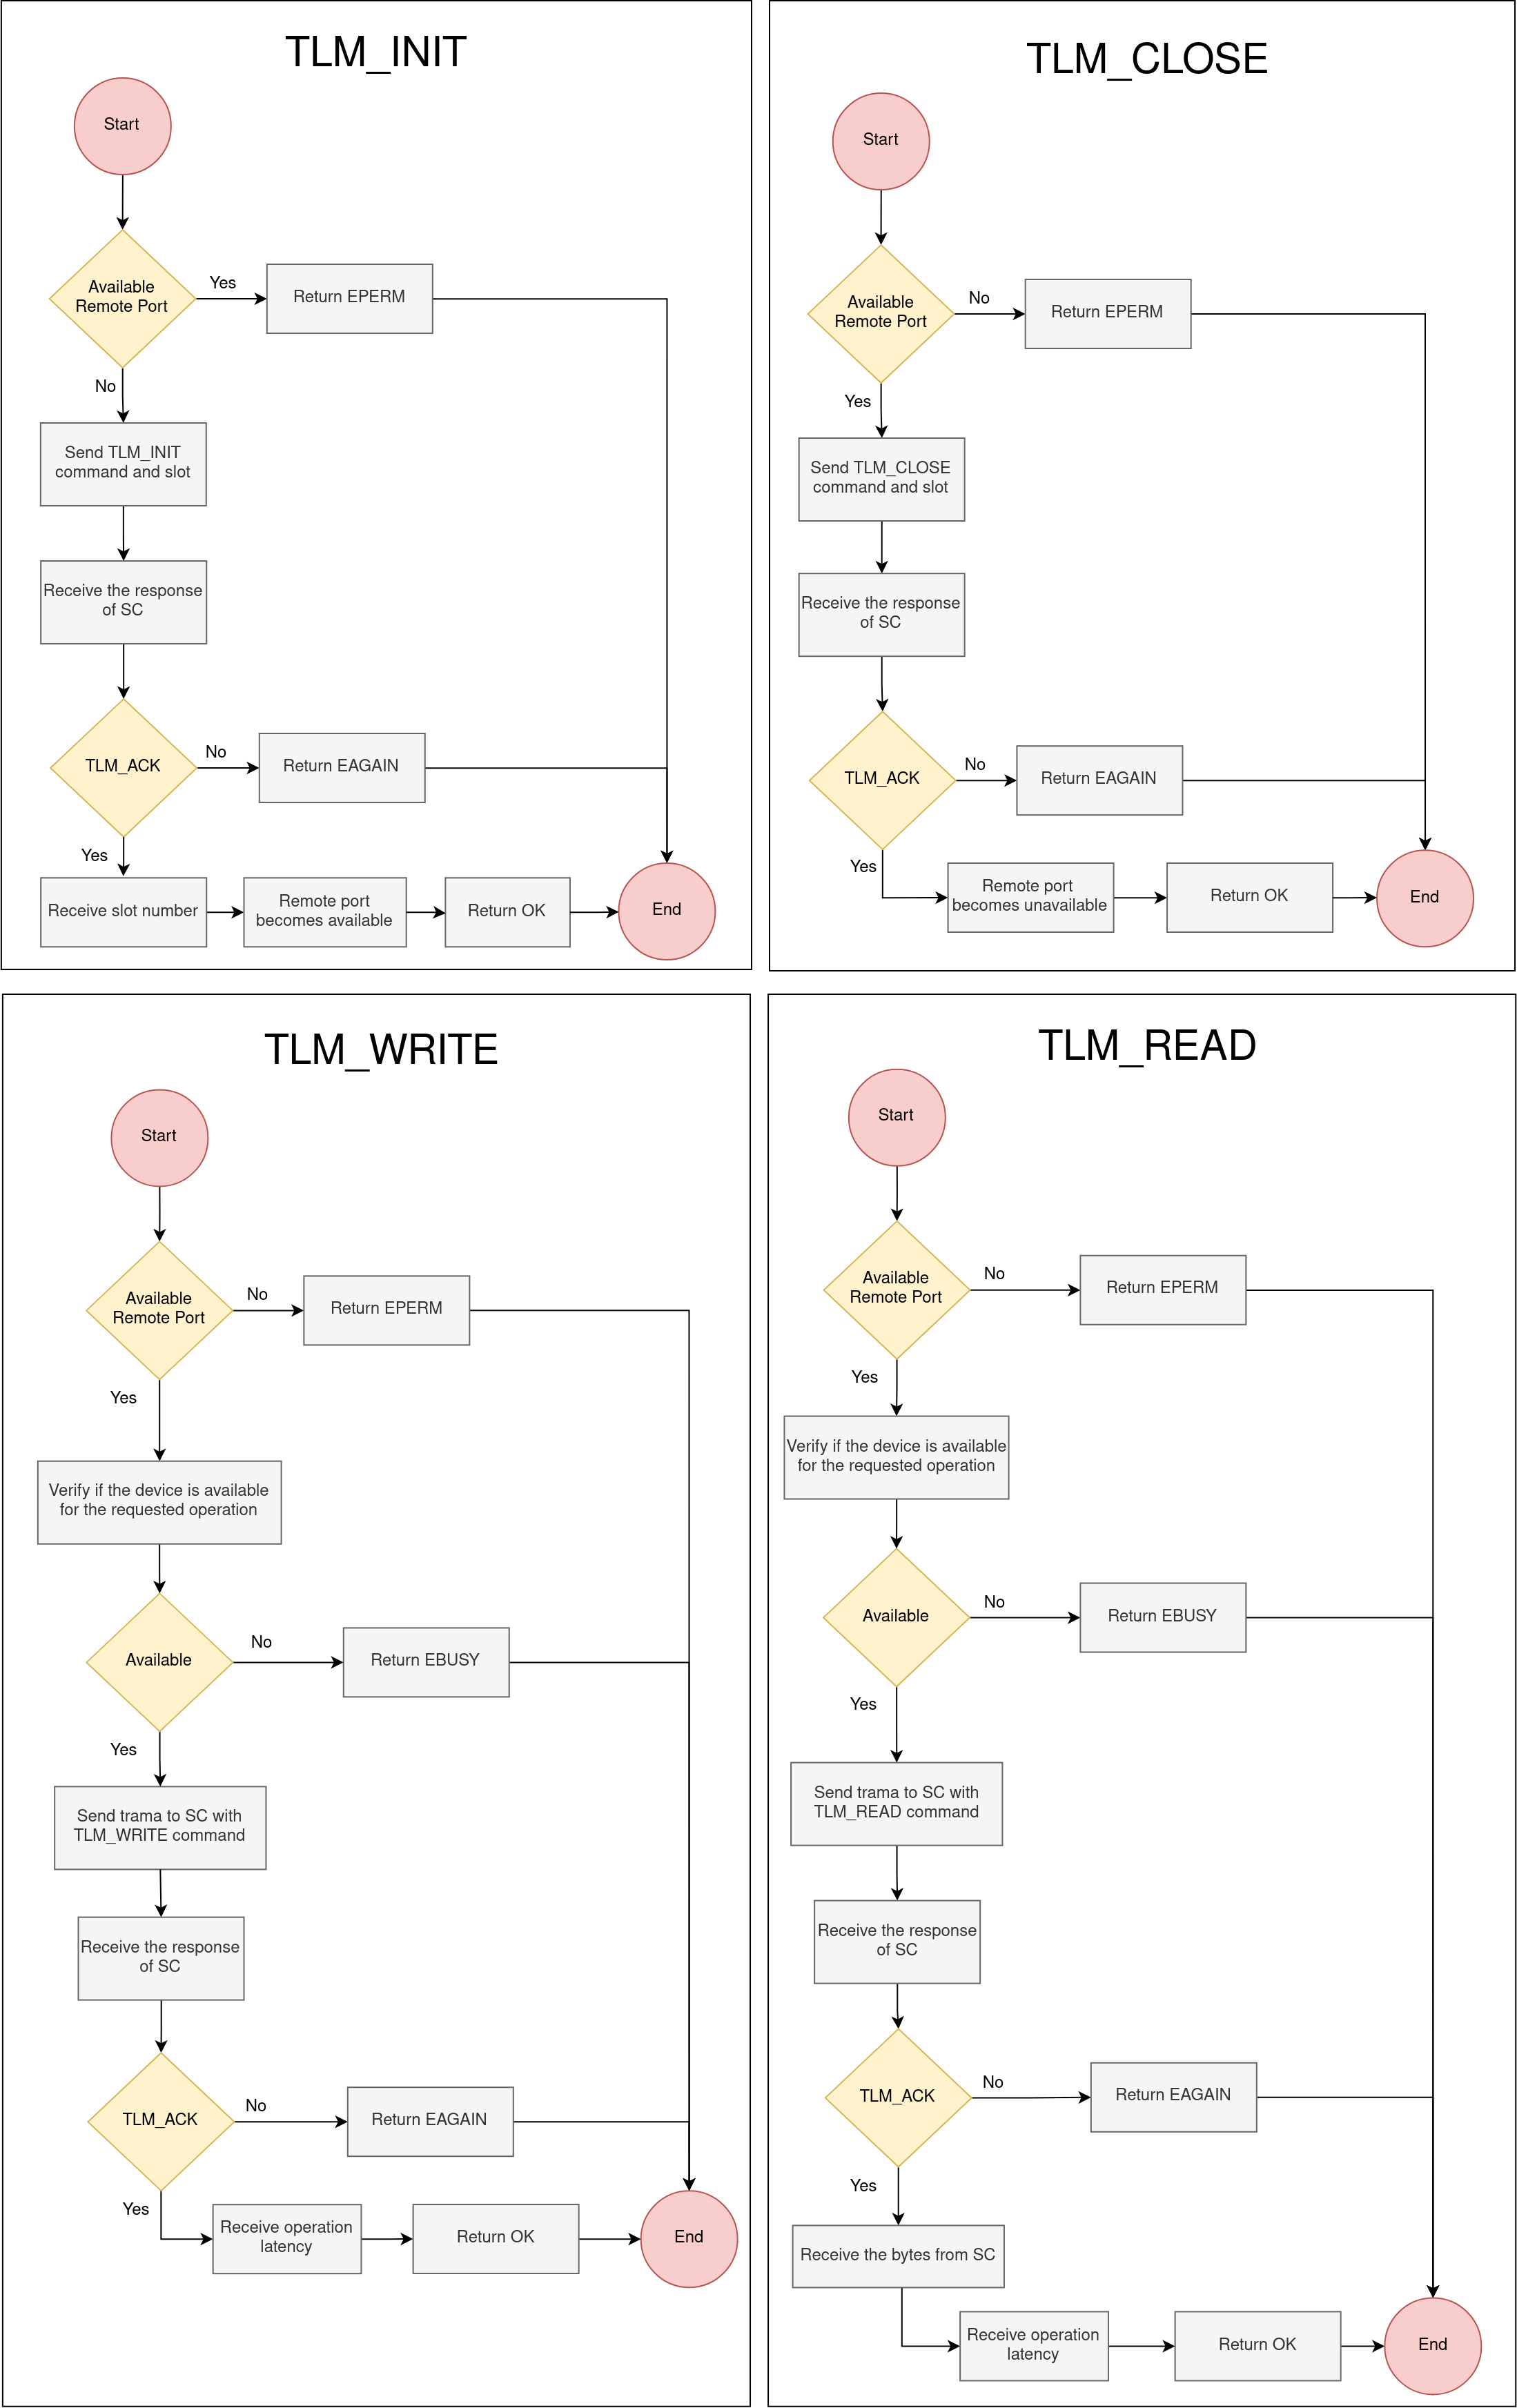
\includegraphics[width=0.8\linewidth]{Images/TLMWrapper_Gem5.png} 
 	\caption{TLM wrapper in Gem5}
	% \label{fig_TLM_Wrapper_Payload}
\end{figure}

\begin{figure}[H]
	\centering
 	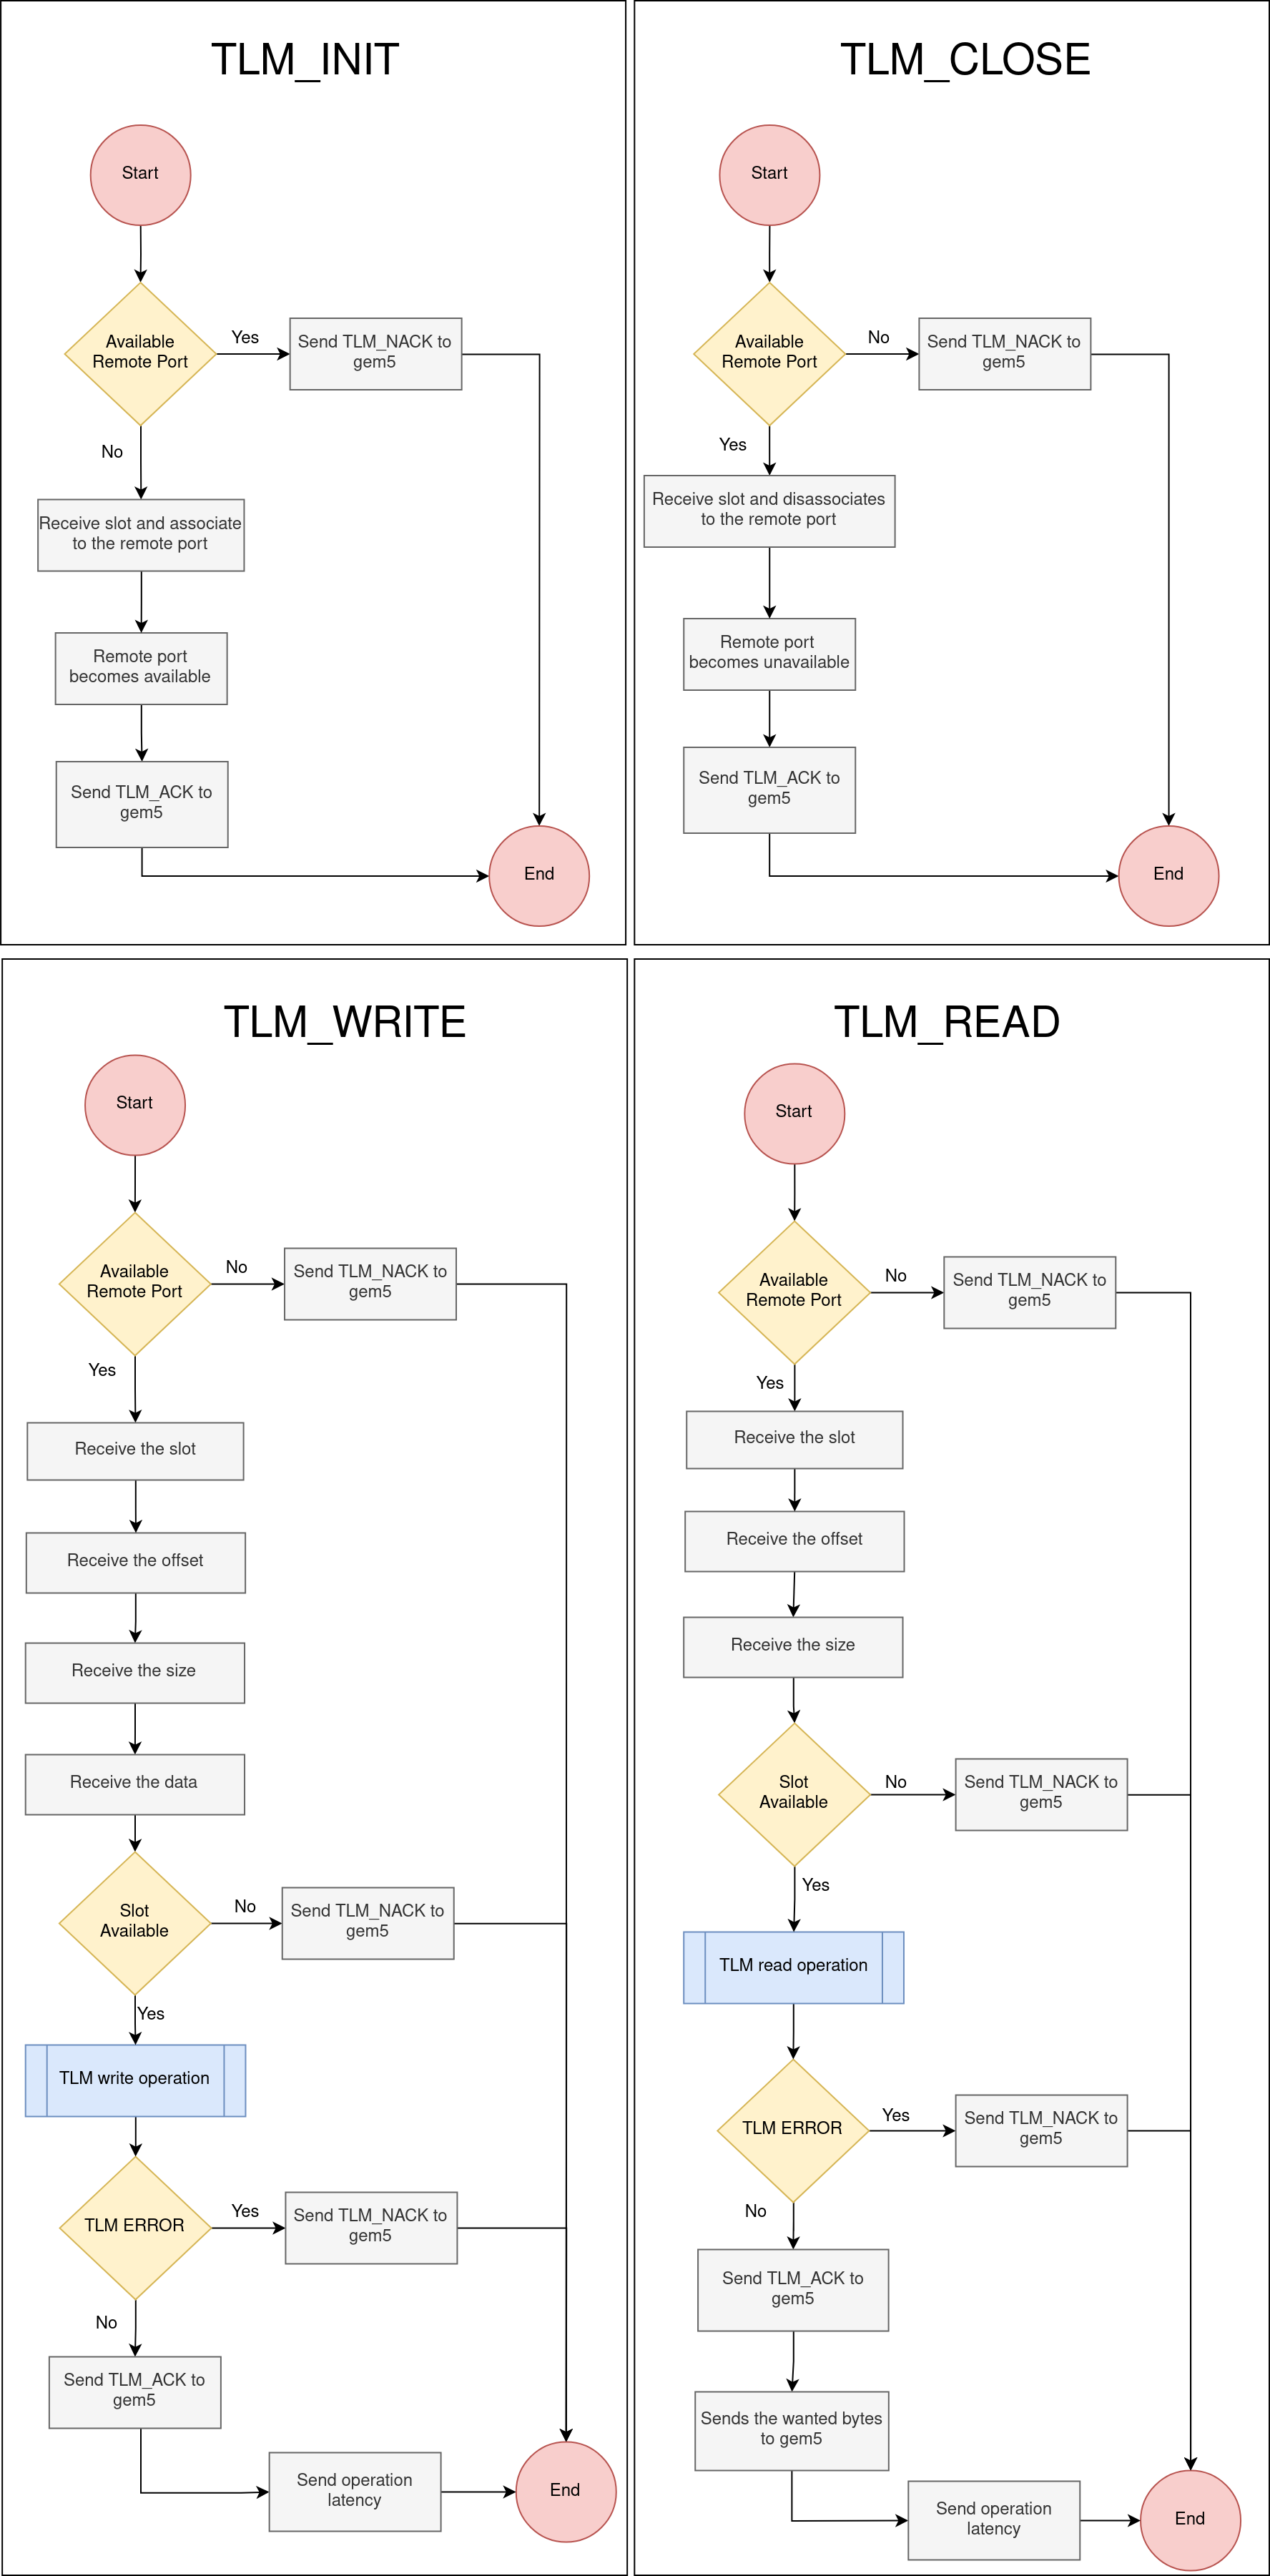
\includegraphics[width=0.7\linewidth]{Images/TLMWrapper_SystemC.png} 
 	\caption{TLM wrapper in SystemC}
	% \label{fig_TLM_Wrapper_Payload}
\end{figure}

\subsection{Application interface}

At this point, the user on the application side can write and read directly from memory without any restriction. However, it can be
dangerous, in the way that the user can, by mistake, do an unpermitted operation. For example, write in reversed memory, causing a
segmentation fault. To avoid this, it was developed an \gls{api} for the application side. Similar to STM32 microcontrollers that 
utilize the HAL library, the \gls{crc} device will also have its own hardware abstraction layer. This layer is designed to expedite 
development and enhance code clarity.

\begin{figure}[H]
	\centering
 	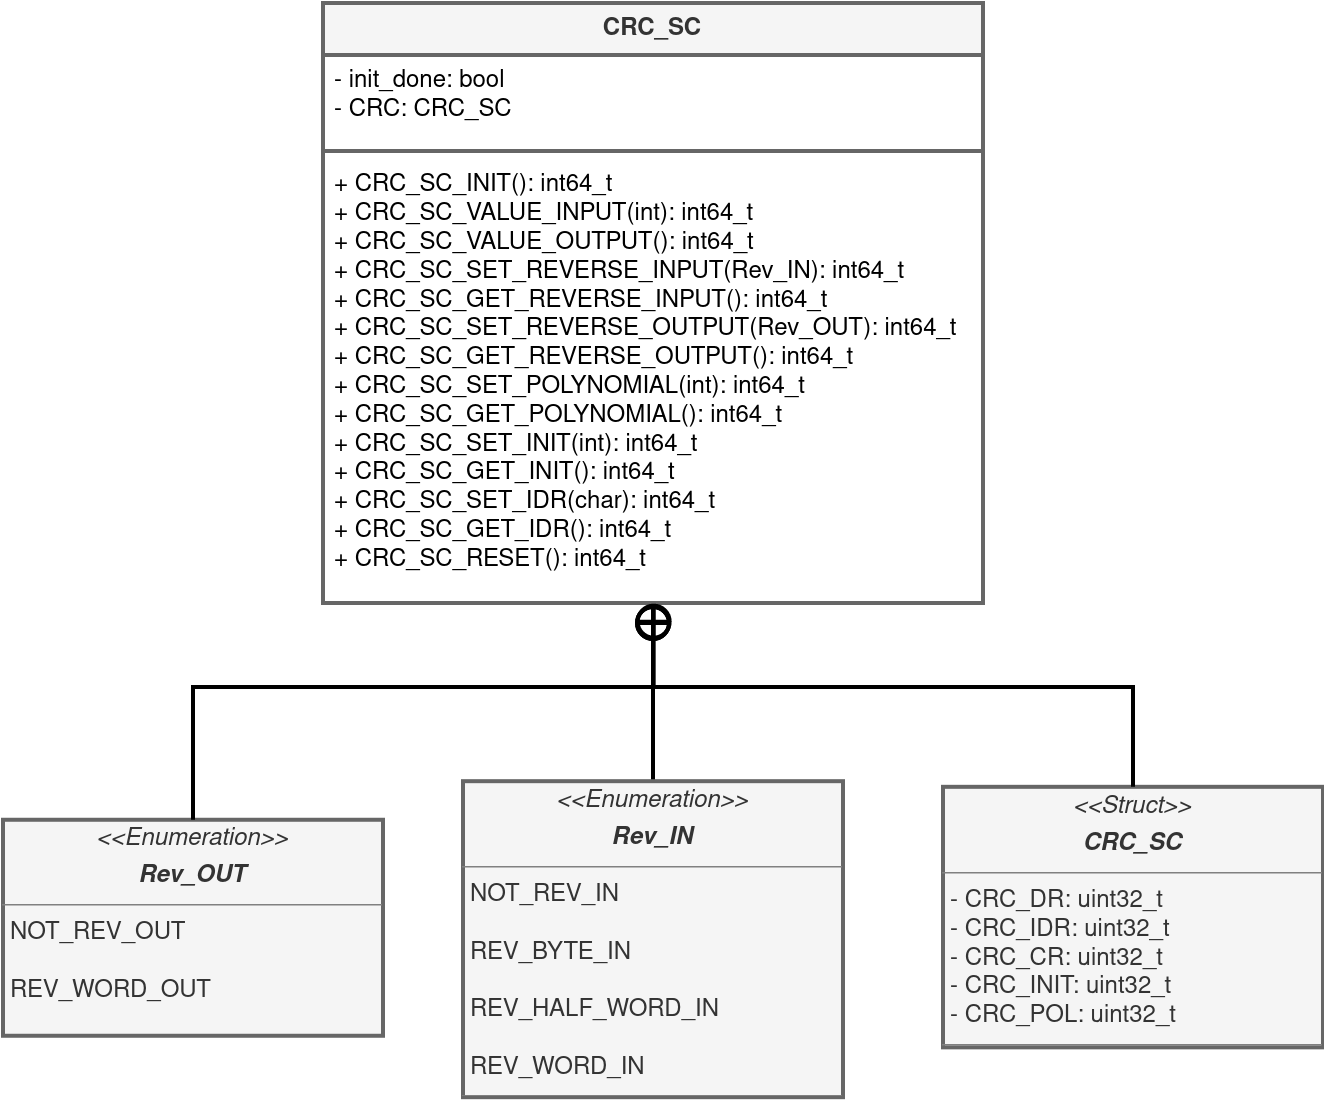
\includegraphics[width=0.7\linewidth]{Images/CRC_API_Class_Diagram.png} 
 	\caption{Class diagram for the \gls{crc} \gls{api}}
	% \label{fig_TLM_Wrapper_Payload}
\end{figure}

Primarily, initializing the peripheral is a mandatory step. Without initialization, any attempt to execute an operation will 
result in an error, and no action will take place. To calculate the \gls{crc} value of a given number, the \textit{CRC\_SC\_VALUE\_INPUT} 
function must be called, with the corresponding number as a parameter. After that, the result can be obtained by calling the 
\textit{CRC\_SC\_VALUE\_OUTPUT} function. It is important to mention that the calculation takes four clock cycles, thus the function can 
either return the \gls{crc} result or an error, warning that the value is not calculated yet. All the remaining functions are used to
control the device.

\section{Application simulation using Gem5}

After the software development, the next step was to simulate and validate it. For this purpose, it was developed a validation test where
all features of the device will be tested. Two cores will be employed for this purpose: one will be dedicated to the 
\gls*{crc}, while the other will execute the bubble-sort benchmark. The simulation will be conducted in sequential mode since 
the main objective is not performance, but accuracy.


\subsection{CRC peripheral validation} 

In order to validate the peripheral, a design of the co-simulation environment was made, as presented in the image 
\ref{fig_CoSimDesign_Validation}. It will be used one \gls*{crc} and the \gls*{uart}, to communicate with the user by the terminal.
As referred, this is already implemented, hence it only requires its initialization and configuration. For the test, it will be used the 
\gls*{uart}0, which is present in the memory map from 0x1C090000 to 0x1C09FFFF.
Regarding the remote connections, each device has one dedicated port. To connect to the \gls*{uart}, the m5term can be utilized. It is
a dedicated program that allows the user to connect to the simulated console interface. When executing the simulation, this program does not
launch automatically, therefore it must be manually called, with \textit{./m5term <host> <port>}.

\begin{figure}[H]
	\centering
 	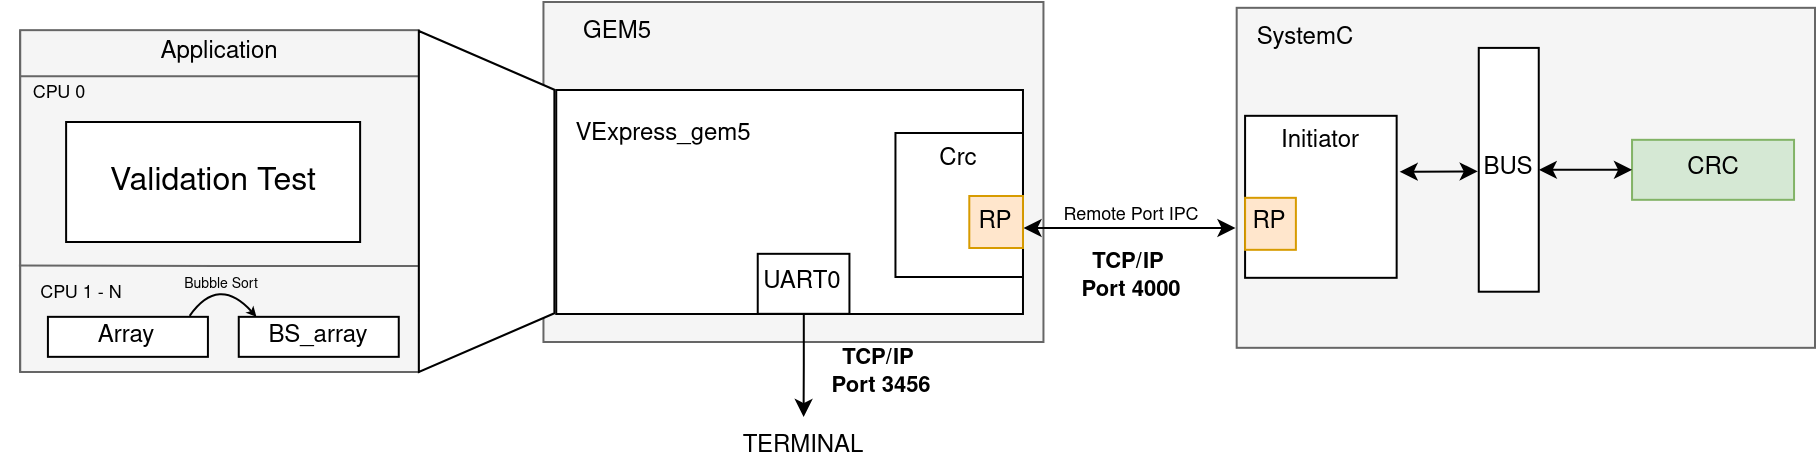
\includegraphics[width=0.8\linewidth]{Images/CoSimDesign_Validation.png} 
 	\caption{Class diagram for the \gls{crc} \gls{api}}
	\label{fig_CoSimDesign_Validation}
\end{figure}

The application will run the code present in \ref{validationCodeCRC}. It can be divided into three parts. In the first one, the reverse 
output will be tested. Then, the settings will change, and the calculation will reserve a reverse input and a different polynomial. To
conclude, the reset function will be checked. By executing this benchmark, every functionality of the peripheral is tested. The expected
outputs are:

\begin{enumerate}
	\item Return from CRC\_DR: 0x22CC4488
	\item Return from CRC\_DR: 0xC66CE444
	\item Reset was done with success! :D
\end{enumerate}

\begin{lstlisting}[language=C, caption={CRC validation code}, label=validationCodeCRC]
CRC_SC_INIT();

CRC_SC_SET_REVERSE_OUTPUT(REV_WORD_OUT);
CRC_SC_SET_IDR(0x4C);
CRC_SC_VALUE_INPUT(0x15e32ef3);       

do //Wait 4 tick
{
	CRC_value = CRC_SC_VALUE_OUTPUT();
} while (CRC_value == -EBUSY);

printf("Return from CRC_DR: %x \n", (uint32_t) CRC_value);

CRC_SC_SET_REVERSE_OUTPUT(NOT_REV_OUT);
CRC_SC_SET_REVERSE_INPUT(REV_HALF_WORD_IN);
CRC_SC_SET_POLYNOMIAL(0x12345678);
CRC_SC_VALUE_INPUT(0x1A2B3C4D);

do //Wait 4 tick
{
	CRC_value = CRC_SC_VALUE_OUTPUT();
} while (CRC_value == -EBUSY);

printf("Return from CRC_DR: %x \n", (uint32_t) CRC_value); 

CRC_SC_SET_INIT(0x4C11DB7);

if(CRC_SC_GET_IDR() == 0x4C)
	CRC_SC_RESET();

if(CRC_SC_VALUE_OUTPUT() == CRC_SC_GET_POLYNOMIAL())
	printf("Reset was done with success! :D\n");
else
	printf("Failure in Reset :L\n");

break;
\end{lstlisting}

After executing the validation benchmark, the real results were the ones present in the \autoref{fig_Validation_Results}. It is possible to conclude that the 
peripheral passed the validation, since every expected output matches the real ones. 

\begin{figure}[H]
	\centering
 	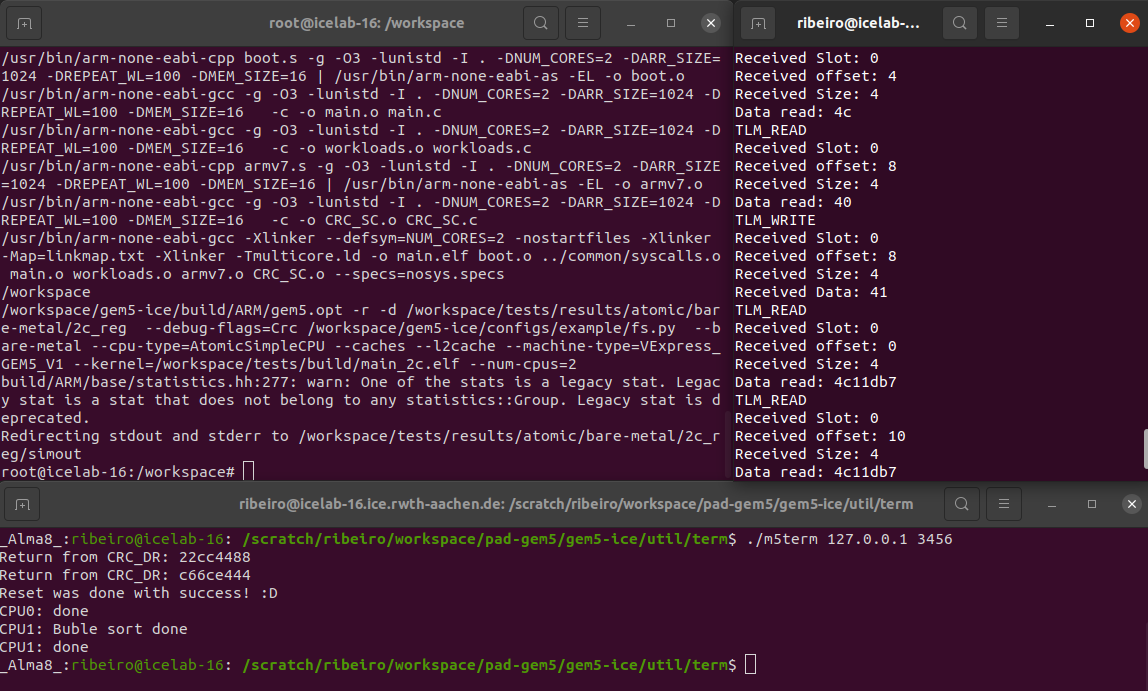
\includegraphics[width=0.8\linewidth]{Images/Validation_Results.png} 
 	\caption{\gls*{crc} validation test results}
	\label{fig_Validation_Results}
\end{figure}


\section{Memory integrity}

With the \gls*{crc}'s validation, it is possible to simulate the scenario as described earlier. Similar to the validation test, 
from the application point of view, the system will execute 2 distinct jobs. \gls{cpu}0 will be responsible for 
performing the memory integrity checks, while the remaining ones will execute a bubble sort algorithm, as presented in 
the \autoref{fig_CoSimDesign}.

\begin{figure}[H]
	\centering
 	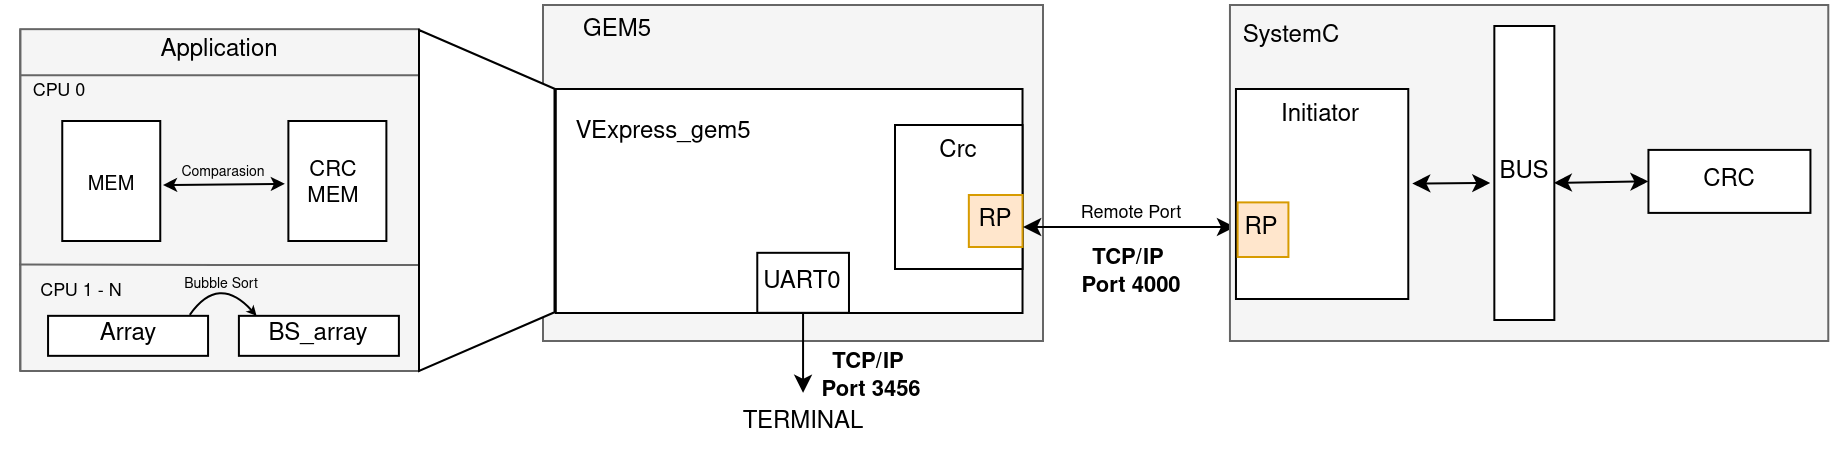
\includegraphics[width=1\linewidth]{Images/CoSimDesign.png}
 	\caption{Co-simulation design}
	 \label{fig_CoSimDesign}
\end{figure}

When the benchmark starts, there is the creation of the intended \glspl{cpu}. Each one has an ID, that allows one to identify
themselves. To conduct the memory integrity test, \gls*{cpu}0 will start initializing the \gls*{crc} and the memory that will 
be utilized to compare. Afterward, periodically, it will perform a memory comparison, having two possible outcomes. Or everything
is alright and the operation is a success. Or there is a flaw and the simulation ends immediately. A detailed view can be 
observed in \ref{fig_MemoryIntegrity_CPU0SequenceDiagram}. 

\begin{figure}[H]
	\centering
 	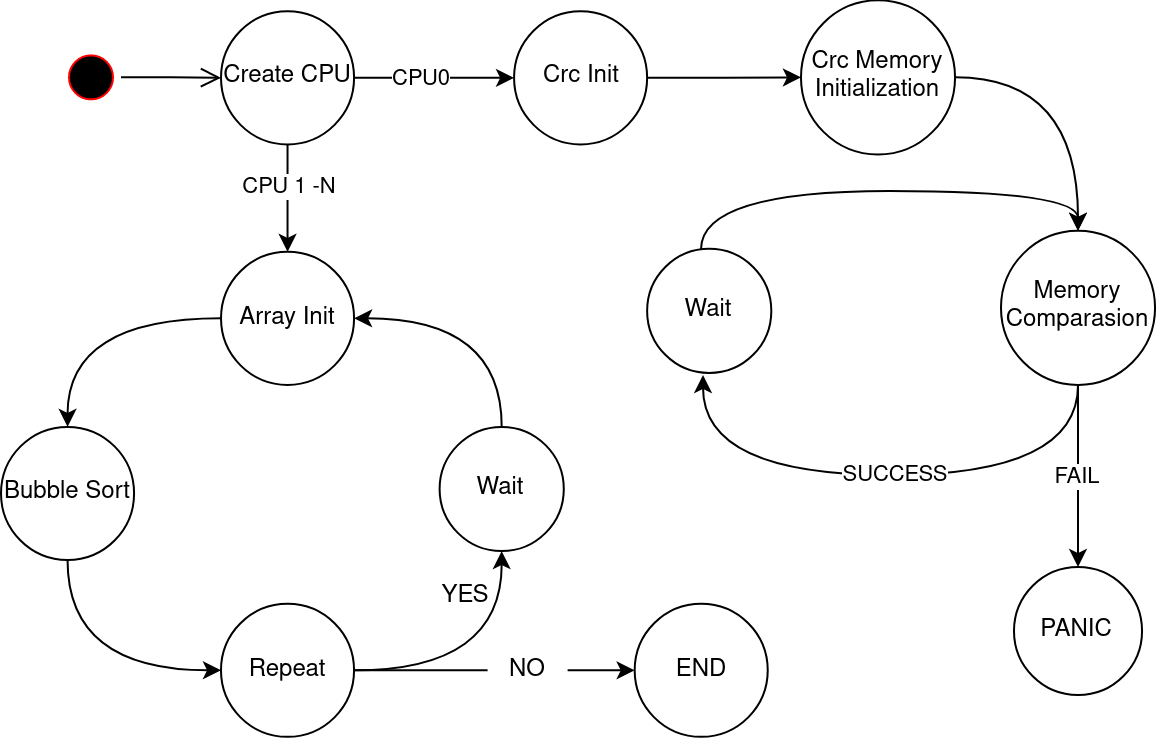
\includegraphics[width=0.7\linewidth]{Images/MemoryIntegrity_StateDiagram.png}
 	\caption{State machine diagram for the memory integrity test}
	\label{fig_MemoryIntegrity_StateDiagram}
\end{figure}

The bubble-sort test run in the remaining instaciated cores. The test will run a pre-defined number of iterations, and 
once all the cores have completed their tasks, the simulation will conclude successfully. At the first moment, the array 
is initialized with random numbers, where the lower and bigger numbers are saved in separate values. Then, the bubble-sort 
the algorithm is executed. To ensure that the simulation ran smoothly, the program compares the first and last values of 
the sorted array with previously saved values. If there is a match, the execution is considered successful. In case of a 
mismatch, a failure is detected, and a notification is sent to the user. However, the simulation continues since the primary 
objective is not to evaluate the bubble-sort algorithm. 

\begin{figure}[H]
	\centering
 	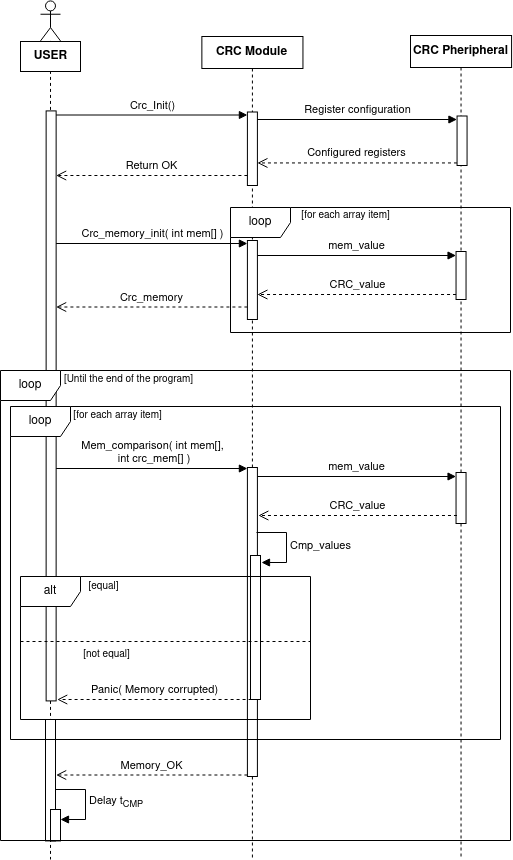
\includegraphics[width=0.7\linewidth]{Images/MemoryIntegrity_CPU0SequenceDiagram.png}
 	\caption{Sequence diagram diagram for the memory comparison}
	\label{fig_MemoryIntegrity_CPU0SequenceDiagram}
\end{figure}

\subsection{Success modeling}

In the first memory integrity test, the perfect scenario will be simulated, in other words, the memory will operate without any failures, 
ensuring a well-functioning system. As represented in the \autoref{fig_MemoryIntegrity_StateDiagram}, there will be an interval between both 
tasks, and this can be different from each other \ref{fig_AppTimeDiagram}. 

\begin{figure}[H]
	\centering
 	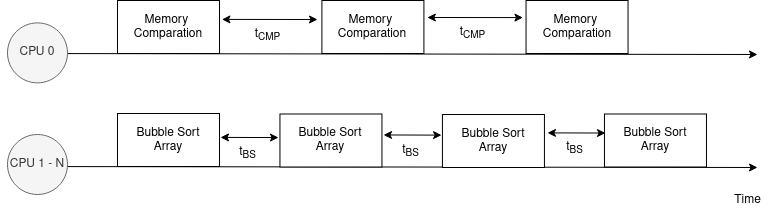
\includegraphics[width=0.8\linewidth]{Images/AppTimeDiagram.png}
 	\caption{Application execution timely diagram}
	 \label{fig_AppTimeDiagram}
\end{figure}


To perform this benchmark, the following parameters were defined. After completing the bubble-sort workload, the system executes a final 
memory check to ensure that no problems occurred between the last one, allowing the simulation to conclude safely. The simulation results are 
available in the subsequent images. As expected, the system executed normally the benchmark without any problems. Both \glspl{cpu} conclude the 
designated tasks and the last memory gives positive feedback. 

\hspace{1.5cm}

\begin{multicols}{2}
	
	\begin{itemize}
		\item Repeat = 100
		\item $t_{CMP}$ = 100 ms
		\item $t_{BS}$ = 10 us
		\item Number of simulated cores = 2
		\item Memory size = 16
	\end{itemize}

	\columnbreak

	\begin{itemize}
		\item Simulation mode = sequential
		\item Reverse input \gls*{crc} = REV\_HALF\_WORD\_IN
		\item Reverse output \gls*{crc} = REV\_WORD\_OUT
		\item Polynomial = 0x04C11DB7
	\end{itemize}

\end{multicols}


\begin{figure}[H]
	\centering
 	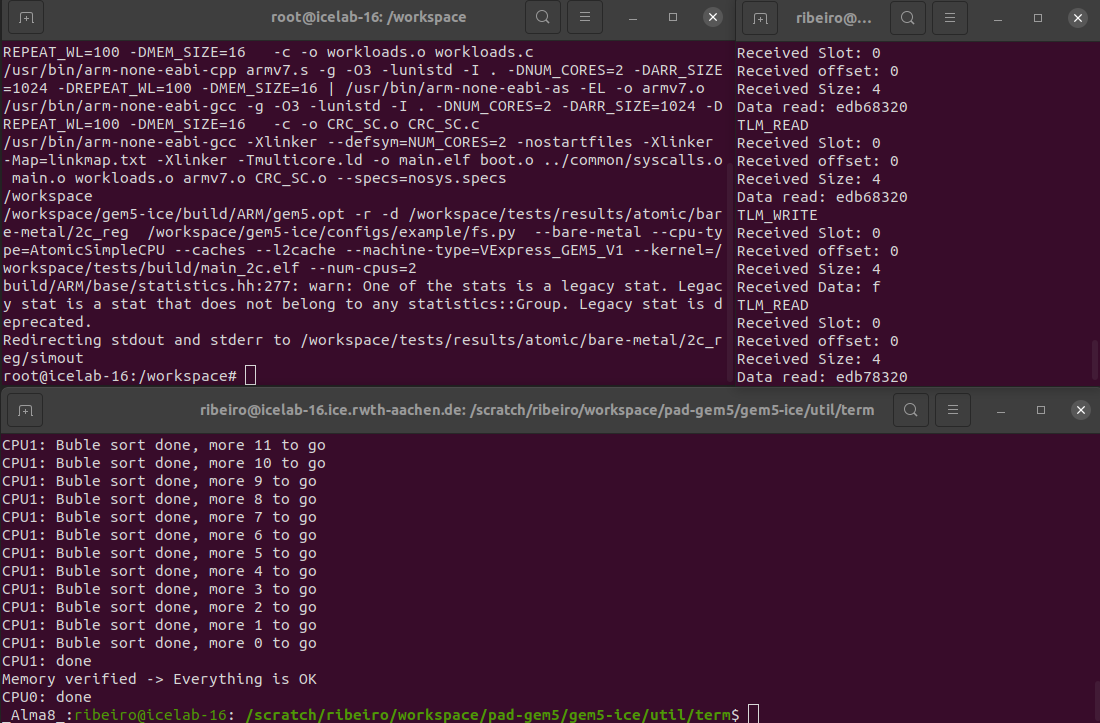
\includegraphics[width=0.8\linewidth]{Images/Success_MemoryIntegrity.png} 
 	\caption{Success memory integrity test}
	%\label{fig_Validation_Results}
\end{figure}


\subsection{Fault modeling}

In opposition to the first, this test will simulate a corrupted memory scenario, as shown in the \autoref{fig_AppTimeDiagramFailure}. 
In order to achieve that, a failure will be injected into the memory with the \gls{gdb} tool. \gls*{gdb} is, as the name suggests, a debugger 
that is supported by Gem5 and SystemC. It offers a variety of features, but for this purpose, the \textit{set} command will be utilized. 
This command allows a value modification of a variable in real time thus, in this way, the failure can be simulated.

\begin{figure}[H]
	\centering
 	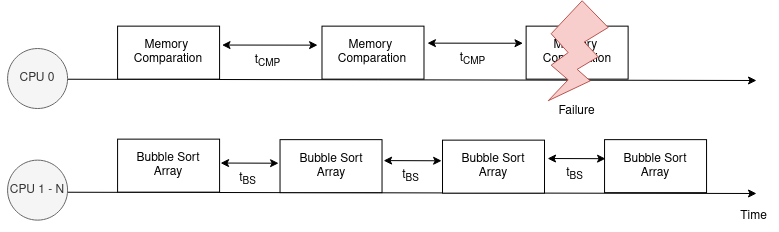
\includegraphics[width=0.8\linewidth]{Images/AppTimeDiagramFailure.png}
 	\caption{Application execution timely diagram with a failure}
	 \label{fig_AppTimeDiagramFailure}
\end{figure}


The test will be done under the same conditions as the previous one nevertheless, in this case, it is expected to end with an error from Gem5. 
It can occur in two different moments. Either when the \gls*{cpu}1-N are still running, or when these already completed their tasks. Both cases  
will be tested, and in either case, the program should terminate promptly. The \autoref{} and \autoref{} demonstrate the obtained results, and 
it can be concluded that the system behaves in accordance with expectations.

\begin{figure}[H]
	\centering
 	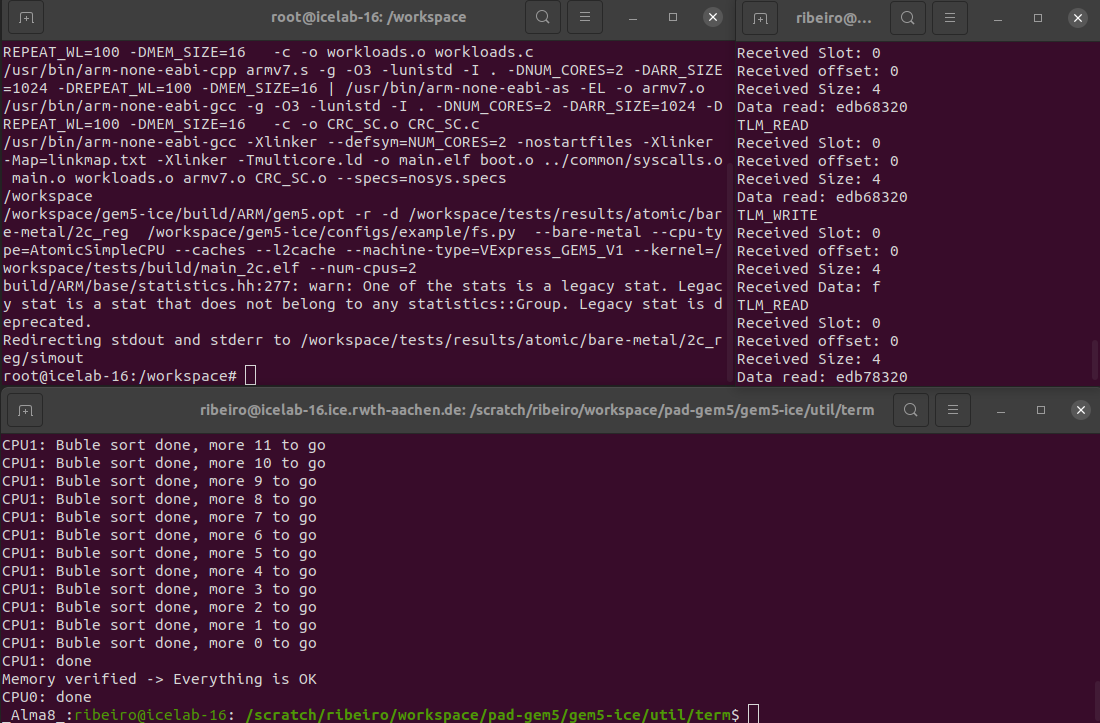
\includegraphics[width=0.8\linewidth]{Images/Success_MemoryIntegrity.png}  %<---- Change to the real ones
 	\caption{Success memory integrity test}
	%\label{fig_Validation_Results}
\end{figure}

\begin{figure}[H]
	\centering
 	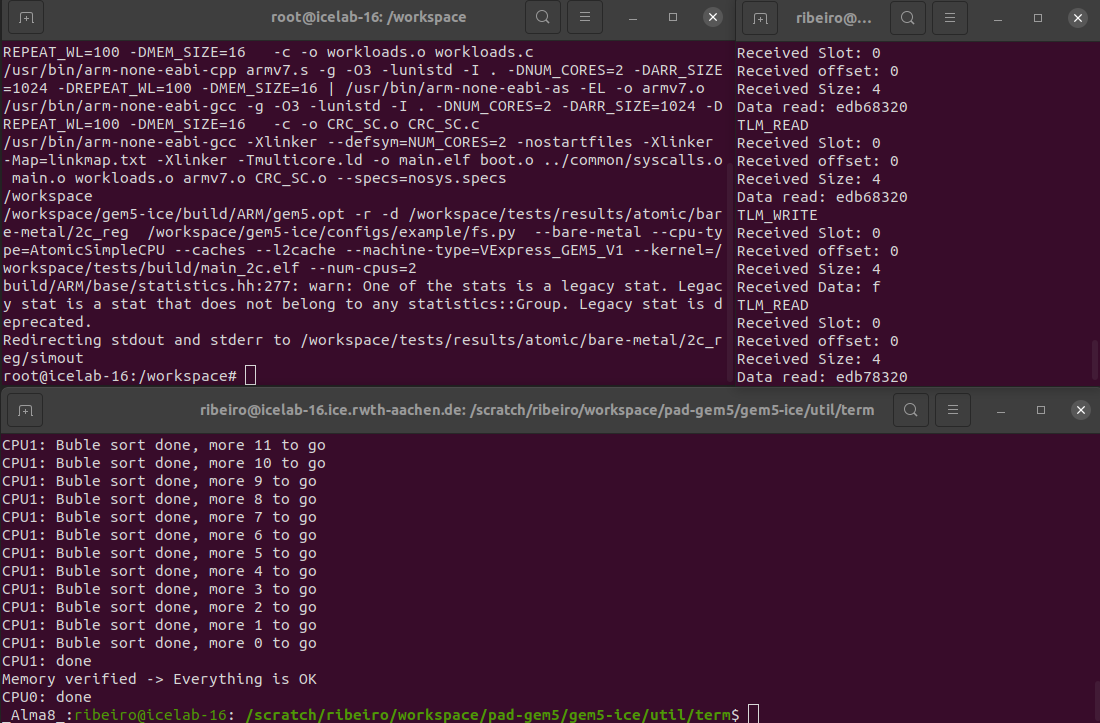
\includegraphics[width=0.8\linewidth]{Images/Success_MemoryIntegrity.png} 
 	\caption{Success memory integrity test}
	%\label{fig_Validation_Results}
\end{figure}


%Mostrar que o sistema reage a falha

\section{Dynamic Quantum}

%Aqui comparar os resultados com o meu algoritmo e sem ele
%Verificarar se houve algum melhoramento

